\documentclass{article}
\usepackage[utf8]{inputenc}
\usepackage{graphicx,caption}
\graphicspath{ {./images/} }
\usepackage{float}
\usepackage{caption}
\usepackage{subcaption}
\usepackage[unicode]{hyperref}
\usepackage{amsmath}

\title{Homework 1 - Theory}
\author{Dainese Fabio, 857661}
\date{March 15, 2020}

\begin{document}

\maketitle

\section{Exercise 1}
    \begin{figure}[H]
        \centering
        \begin{minipage}[b]{0.25\textwidth}
            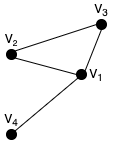
\includegraphics[width=\textwidth]{1.png}
            \subcaption{Undirected graph}
            \label{fig:figure-1-a}
        \end{minipage}
        \hfill
        \begin{minipage}[b]{0.5\textwidth}
            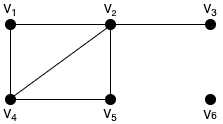
\includegraphics[width=\textwidth]{2.png}
            \subcaption{Undirected graph}
            \label{fig:figure-1-b}
        \end{minipage}
        \label{fig:figure-1}
    \end{figure}
    
    \subsection{Answers About Graph 'a'}
    The degree of each vertex is:
    \begin{align*}
    d(v_{1}) &= |N(v_{1})|-1 =|\{v_{1},v_{2},v_{3},v_{4}\}|-1 = 4 - 1 = 3\\
    d(v_{2}) &= |N(v_{2})|-1 =|\{v_{1},v_{2},v_{3}\}|-1 = 3 - 1 = 2\\
    d(v_{3}) &= |N(v_{3})|-1 =|\{v_{1},v_{2},v_{3}\}|-1 = 3 - 1 = 2 \\
    d(v_{4}) &= |N(v_{4})|-1 =|\{v_{1},v_{4}\}|-1 = 2 - 1 = 1
    \end{align*}

    \par\noindent The even vertices are \(\{v_{2},v_{3}\}\).\newline
    
    \par\noindent The average degree is:
    \[
    Ad(G) = \frac{1}{|V|} \sum_{v \in V} d(v) = \frac{1}{4} \cdot (3+2+2+1) = \frac{1}{4} \cdot 8 = 2
    \]
    
    \subsection{Answers About Graph 'b'}
    The degree of each vertex is:
    \begin{align*}
    d(v_{1}) &= |N(v_{1})|-1 =|\{v_{1},v_{2},v_{4}\}|-1 = 3 - 1 = 2\\
    d(v_{2}) &= |N(v_{2})|-1 =|\{v_{1},v_{2},v_{3},v_{4},v_{5}\}|-1 = 5 - 1 = 4\\
    d(v_{3}) &= |N(v_{3})|-1 =|\{v_{2},v_{3}\}|-1 = 2 - 1 = 1 \\
    d(v_{4}) &= |N(v_{4})|-1 =|\{v_{1},v_{2},v_{4},v_{5}\}|-1 = 4 - 1 = 3 \\
    d(v_{5}) &= |N(v_{5})|-1 =|\{v_{2},v_{4},v_{5}\}|-1 = 3 - 1 = 2 \\
    d(v_{6}) &= 0
    \end{align*}

    \par\noindent The even vertices are \(\{v_{1},v_{2},v_{5},v_{6}\}\).\newline
    
    \par\noindent The average degree is:
    \[
    Ad(G) = \frac{1}{|V|} \sum_{v \in V} d(v) = \frac{1}{6} \cdot (2+4+1+3+2+0) = \frac{1}{6} \cdot 12 = 2
    \]
    
\section{Exercise 2}
    \begin{figure}[H]
        \centering
        \begin{minipage}[b]{0.3\textwidth}
            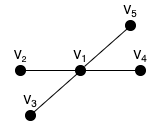
\includegraphics[width=\textwidth]{3.png}
            \subcaption{Undirected graph}
            \label{fig:figure-2-a}
        \end{minipage}
        \hfill
        \begin{minipage}[b]{0.5\textwidth}
            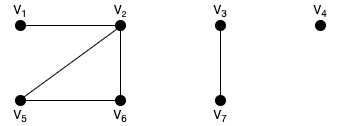
\includegraphics[width=\textwidth]{4.png}
            \subcaption{Undirected graph}
            \label{fig:figure-2-b}
        \end{minipage}
        \label{fig:figure-2}
    \end{figure}
    
    \subsection{Answers About Graph 'a'}
    There aren't isolated vertices (i.e. vertices with \(d(v)=0\)).\newline
    
    \par\noindent The graph is not complete (proof by counterexample: \(v_{2}\) and \(v_{5}\) are not adjacent).\newline
    
    \par\noindent A path from \(v_{1}\) to \(v_{5}\) is \{\(e_{1}\)\}, where \(e_{1} = \{v_{1},v_{5}\}\).\newline
    
    \par\noindent The graphs is connected since there exists a path from \(v\) to \(w\), \(\forall v,w \in V\).\newline
    
    \par\noindent The connected components of \(v_{1}\) and \(v_{3}\) are:
    \[
    C_{v_{1}} = C_{v_{3}} = \{v_{1},v_{2},v_{3},v_{4},v_{5}\}
    \]
    \newline
    
    \par\noindent The adjacent matrix associated to the graph is:
    \begin{equation*}
    A =
        \begin{bmatrix}
        0 & 1 & 1 & 1 & 1\\
        1 & 0 & 0 & 0 & 0\\
        1 & 0 & 0 & 0 & 0\\
        1 & 0 & 0 & 0 & 0\\
        1 & 0 & 0 & 0 & 0\\
        \end{bmatrix}
    \end{equation*}
    
    \subsection{Answers About Graph 'b'}
    There's only one isolated vertex and that is \(v_{4}\), since \(d(v_{4})=0\).\newline
    
    \par\noindent The graph is not complete (proof by counterexample: \(v_{1}\) and \(v_{5}\) are not adjacent).\newline
    
    \par\noindent A path from \(v_{1}\) to \(v_{5}\) is \{\(e_{1},e_{2}\)\}, where \(e_{1} = \{v_{1},v_{2}\}\) and \(e_{2} = \{v_{2},v_{5}\}\).\newline
    
    \par\noindent The graphs is not connected since there's not exists a path from \(v\) to \(w\), \(\forall v,w \in V\), for example from \(v_{2}\) and \(v_{3}\).\newline
    
    \par\noindent The connected components of \(v_{1}\) and \(v_{3}\) are:
    \begin{align*}
    C_{v_{1}} &= \{v_{1},v_{2},v_{5},v_{6}\} \\
    C_{v_{3}} &= \{v_{3},v_{7}\}
    \end{align*}
    
    \par\noindent The adjacent matrix associated to the graph is:
    \begin{equation*}
    A =
        \begin{bmatrix}
        0 & 1 & 0 & 0 & 0 & 0 & 0\\
        1 & 0 & 0 & 0 & 1 & 1 & 0\\
        0 & 0 & 0 & 0 & 0 & 0 & 1\\
        0 & 0 & 0 & 0 & 0 & 0 & 0\\
        0 & 1 & 0 & 0 & 0 & 1 & 0\\
        0 & 1 & 0 & 0 & 1 & 0 & 0\\
        0 & 0 & 1 & 0 & 0 & 0 & 0\\
        \end{bmatrix}
    \end{equation*}
    
\section{Exercise 3}
    \begin{figure}[H]
        \centering
        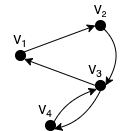
\includegraphics[width=0.3\textwidth]{5.png}
        \caption{Directed graph}
        \label{fig:figure-3}
    \end{figure}
    
    The vertex set of the graph is: \[V=\{v_{1},v_{2},v_{3},v_{4}\}\]
    
    \par\noindent The edge set of the graph is:
    \[E=\{(v_{1},v_{2}),(v_{2},v_{3}),(v_{3},v_{1}),(v_{3},v_{4}),(v_{4},v_{3})\}\]
    
    \par\noindent The adjacent matrix associated to the graph is:
    \begin{equation*}
    A =
        \begin{bmatrix}
        0 & 1 & 0 & 0\\
        0 & 0 & 1 & 0\\
        1 & 0 & 0 & 1\\
        0 & 0 & 1 & 0\\
        \end{bmatrix}
    \end{equation*}
    
    \par\noindent The in (\(d^{+}(v)\)), out (\(d^{-}(v)\)) and total degree (\(d(v)\)) of each node is:
    \begin{align*}
    d^{+}(v_{1}) &= |N^{+}(v_{1})|-1 = |\{v_{1},v_{3}\}|-1 = 2-1 = 1\\
    d^{-}(v_{1}) &= |N^{-}(v_{1})|-1 = |\{v_{1},v_{2}\}|-1 = 2-1 = 1\\
    d(v_{1}) &= d^{+}(v_{1}) + d^{-}(v_{1}) = 1+1 = 2\\\\
    d^{+}(v_{2}) &= |N^{+}(v_{2})|-1 = |\{v_{1},v_{2}\}|-1 = 2-1 = 1\\
    d^{-}(v_{2}) &= |N^{-}(v_{2})|-1 = |\{v_{2},v_{3}\}|-1 = 2-1 = 1\\
    d(v_{2}) &= d^{+}(v_{2}) + d^{-}(v_{2}) = 1+1 = 2\\\\
    \end{align*}
    \begin{align*}
    d^{+}(v_{3}) &= |N^{+}(v_{3})|-1 = |\{v_{2},v_{3},v_{4}\}|-1 = 3-1 = 2\\
    d^{-}(v_{3}) &= |N^{-}(v_{3})|-1 = |\{v_{1},v_{3},v_{4}\}|-1 = 3-1 = 2\\
    d(v_{3}) &= d^{+}(v_{3}) + d^{-}(v_{3}) = 2+2 = 4\\\\
    d^{+}(v_{4}) &= |N^{+}(v_{4})|-1 = |\{v_{3},v_{4}\}|-1 = 2-1 = 1\\
    d^{-}(v_{4}) &= |N^{-}(v_{4})|-1 = |\{v_{3},v_{4}\}|-1 = 2-1 = 1\\
    d(v_{4}) &= d^{+}(v_{4}) + d^{-}(v_{4}) = 1+1 = 2\\\\
    \end{align*}
    
    \par\noindent One of many possible paths that can be found in the graph is for example the one from \(v_{1}\) to \(v_{3}\) defined as \((e_{1},e_{2})\), where \(e_{1}=(v_{1},v_{2})\) and \(e_{2}=(v_{2},v_{3})\).

\section{Exercise 4}
    \begin{figure}[H]
        \centering
        \begin{minipage}[b]{0.5\textwidth}
            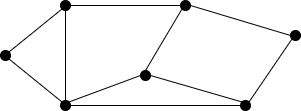
\includegraphics[width=\textwidth]{6.png}
            \label{fig:figure-4-a}
        \end{minipage}
        \hfill
        \begin{minipage}[b]{0.4\textwidth}
            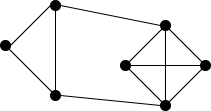
\includegraphics[width=\textwidth]{7.png}
            \label{fig:figure-4-b}
        \end{minipage}
        \label{fig:figure-1}
    \end{figure}
    
    These two graphs are not isomorphic. In this case a simple way to prove it is to compare the list of vertex degree of the two given graphs.
    
    \begin{align*}
        G_{1} &= \{2,2,3,3,3,3,4\}\\
        G_{2} &= \{2,3,3,3,3,4,4\}
    \end{align*}
    
    \noindent As you can see \(G_{1}\) and \(G_{2}\) are not identical, thus the two graphs are not isomorphic.\newline
    Another simpler way to prove it is to compare the cardinalities of the two edge sets, i.e. \(|E_{1}| \neq |E_{2}| \implies\) No isomorphic.
    
\section{Exercise 5}
    \begin{figure}[H]
        \centering
        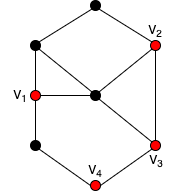
\includegraphics[width=0.35\textwidth]{8.png}
        \label{fig:figure-5}
    \end{figure}
    
    The distances, i.e. the minimum path length between two vertices, of \(d(v_{1},v_{2})\), \(d(v_{1},v_{3})\) and \(d(v_{1},v_{4})\) are all equal to 2.\newline
    
    \par\noindent The diameter of the given graph is equals to 3, recalling that the diameter is the maximum between all the possible distances of the graph's vertices.\newline
    
    \par\noindent The centers of the given graphs are \(v_{1}\), \(v_{3}\) and the middle vertex (the 'inside' vertex), recalling that a vertex \(u\) is a centre of a graph \(G\) if its maximum distance from any other vertex \(v\) is minimum.\newline
    
    \par\noindent The radius of this graph is equals to 2 (maximum distance between the centers and the rest of the vertices).
    
\section{Exercise 6}
    \begin{figure}[H]
        \centering
        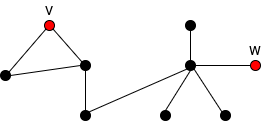
\includegraphics[width=0.7\textwidth]{9.png}
        \label{fig:figure-6}
    \end{figure}
    
    In the given graph there are three cut points as shown in the following images (red vertices):
    
    \begin{figure}[H]
        \centering
        \begin{minipage}[b]{0.4\textwidth}
            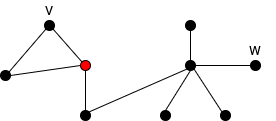
\includegraphics[width=\textwidth]{9.1.png}
            \label{fig:figure-6-1}
        \end{minipage}
        \hfill
        \begin{minipage}[b]{0.4\textwidth}
            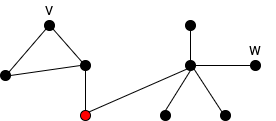
\includegraphics[width=\textwidth]{9.2.png}
            \label{fig:figure-6-2}
        \end{minipage}
        \hfill
        \begin{minipage}[b]{0.4\textwidth}
            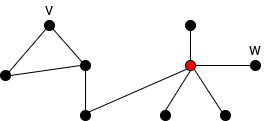
\includegraphics[width=\textwidth]{9.3.png}
            \label{fig:figure-6-3}
        \end{minipage}
    \end{figure}
    
    \noindent By removing the first cut point, we obtain the following situation:
    \begin{figure}[H]
        \centering
        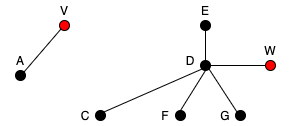
\includegraphics[width=0.5\textwidth]{9.4.png}
        \label{fig:figure-6-4}
    \end{figure}
    \noindent In this configuration the connected component of \(v\) and \(w\) are:
    \begin{align*}
        C_{v} &= \{A,V\}\\
        C_{w} &= \{C,D,E,F,G,W\}
    \end{align*}
    
    \noindent Meanwhile if we remove the second cut point, we obtain the following situation:
    \begin{figure}[H]
        \centering
        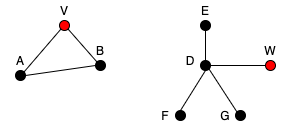
\includegraphics[width=0.5\textwidth]{9.5.png}
        \label{fig:figure-6-5}
    \end{figure}
    \noindent In this configuration the connected component of \(v\) and \(w\) are:
    \begin{align*}
        C_{v} &= \{A,B,V\}\\
        C_{w} &= \{D,E,F,G,W\}
    \end{align*}
    
    \noindent Finally if we remove the third cut point, we obtain the following situation:
    \begin{figure}[H]
        \centering
        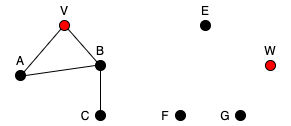
\includegraphics[width=0.5\textwidth]{9.6.png}
        \label{fig:figure-6-6}
    \end{figure}
    \noindent In this configuration the connected component of \(v\) and \(w\) are:
    \begin{align*}
        C_{v} &= \{A,B,C,V\}\\
        C_{w} &= \{W\}
    \end{align*}
    
\section{Exercise 7}
    \begin{figure}[H]
        \centering
        \begin{minipage}[b]{0.2\textwidth}
            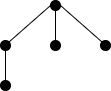
\includegraphics[width=\textwidth]{10.1.png}
            \subcaption{}
            \label{fig:figure-7-1}
        \end{minipage}
        \hfill
        \begin{minipage}[b]{0.3\textwidth}
            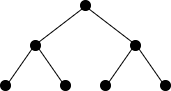
\includegraphics[width=\textwidth]{10.2.png}
            \subcaption{}
            \label{fig:figure-7-2}
        \end{minipage}
        \hfill
        \begin{minipage}[b]{0.4\textwidth}
            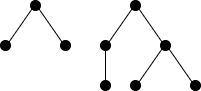
\includegraphics[width=\textwidth]{10.3.png}
            \subcaption{}
            \label{fig:figure-7-3}
        \end{minipage}
    \end{figure}
    
    The \(a\) and \(b\) graphs are trees.\newline
    \par\noindent The \(a\),\(b\) and \(c\) graphs are forests.\newline
    \par\noindent The \(b\) graph is a binary tree. Also \(a\) can be a binary three if we consider as a root the middle node.\newline
    
\section{Exercise 8}
    \begin{figure}[H]
        \centering
        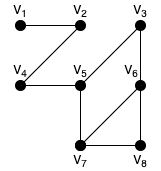
\includegraphics[width=0.35\textwidth]{11.png}
        \label{fig:figure-8}
    \end{figure}
    
    The adjacent matrix of the graph is:
    \begin{equation*}
    A =
        \begin{bmatrix}
        0 & 1 & 0 & 0 & 0 & 0 & 0 & 0\\
        1 & 0 & 0 & 1 & 0 & 0 & 0 & 0\\
        0 & 0 & 0 & 0 & 1 & 1 & 0 & 0\\
        0 & 1 & 0 & 0 & 1 & 0 & 0 & 0\\
        0 & 0 & 1 & 1 & 0 & 0 & 1 & 0\\
        0 & 0 & 1 & 0 & 0 & 0 & 1 & 1\\
        0 & 0 & 0 & 0 & 1 & 1 & 0 & 1\\
        0 & 0 & 0 & 0 & 0 & 1 & 1 & 0\\
        \end{bmatrix}
    \end{equation*}
    
    \noindent The number of chains of length 2 and 4 are:
    \begin{align*}
        A^{2} = A \cdot A &= 
        \begin{bmatrix}
        1 & 0 & 0 & 1 & 0 & 0 & 0 & 0\\
        0 & 2 & 0 & 0 & 1 & 0 & 0 & 0\\
        0 & 0 & 2 & 1 & 0 & 0 & 2 & 1\\
        1 & 0 & 1 & 2 & 0 & 0 & 1 & 0\\
        0 & 1 & 0 & 0 & 3 & 2 & 0 & 1\\
        0 & 0 & 0 & 0 & 2 & 3 & 1 & 1\\
        0 & 0 & 2 & 1 & 0 & 1 & 3 & 1\\
        0 & 0 & 1 & 0 & 1 & 1 & 1 & 2
        \end{bmatrix}\\
        A^{4} = A \cdot A \cdot A \cdot A &= 
        \begin{bmatrix}
        2 & 0 & 1 & 3 & 0 & 0 & 1 & 0\\
        0 & 5 & 0 & 0 & 5 & 2 & 0 & 1\\
        1 & 0 & 10 & 6 & 1 & 3 & 12 & 6\\
        3 & 0 & 6 & 7 & 0 & 1 & 7 & 2\\
        0 & 5 & 1 & 0 & 15 & 13 & 3 & 7\\
        0 & 2 & 3 & 1 & 13 & 15 & 7 & 8\\
        1 & 0 & 12 & 7 & 3 & 7 & 16 & 8\\
        0 & 1 & 6 & 2 & 7 & 8 & 8 & 8
        \end{bmatrix}
    \end{align*}
    
    \noindent Which, by summing all the elements of \(A^{2}\) gives 44 possible chains of length 2, meanwhile by summing all the elements of \(A^{4}\) gives 272 possible chains of length 4.\newline
    
    \par\noindent Assuming the given bijection \(\phi\) of the task, the resulting permutation matrix \(P_{\phi}\) is:
    
    \[
    P_{\phi}=
    \begin{bmatrix}
        0 & 1 & 0 & 0 & 0 & 0 & 0 & 0\\
        1 & 0 & 0 & 0 & 0 & 0 & 0 & 0\\
        0 & 0 & 1 & 0 & 0 & 0 & 0 & 0\\
        0 & 0 & 0 & 1 & 0 & 0 & 0 & 0\\
        0 & 0 & 0 & 0 & 0 & 1 & 0 & 0\\
        0 & 0 & 0 & 0 & 1 & 0 & 0 & 0\\
        0 & 0 & 0 & 0 & 0 & 0 & 1 & 0\\
        0 & 0 & 0 & 0 & 0 & 0 & 0 & 1\\
    \end{bmatrix}
    \]
    
    \noindent As before to calculate the chains of length 2 and 4 of the relabelled graph we need to perform \(\widetilde{A^{2}}\) and \(\widetilde{A^{4}}\), which gives 44 possible chains of length 2 and 272 of length 4 (as before). To recall that now the adjacent matrix is: 
    \[
    \widetilde{A}=
    \begin{bmatrix}
        0 & 1 & 0 & 1 & 0 & 0 & 0 & 0\\
        1 & 0 & 0 & 0 & 0 & 0 & 0 & 0\\
        0 & 0 & 0 & 0 & 1 & 1 & 0 & 0\\
        1 & 0 & 0 & 0 & 0 & 1 & 0 & 0\\
        0 & 0 & 1 & 0 & 0 & 0 & 1 & 1\\
        0 & 0 & 1 & 1 & 0 & 0 & 1 & 0\\
        0 & 0 & 0 & 0 & 1 & 1 & 0 & 1\\
        0 & 0 & 0 & 0 & 1 & 0 & 1 & 0\\
    \end{bmatrix}
    \]
    
\section{Exercise 9}
By defining a "Null Graph" as a graph \(G=(V,E)\) with \(n\) vertices and \(E = \O\), we have:

\begin{itemize}
    \item The number of edges equal to zero (\(|E|=0\));
    \item Only 1 face (outer face/region);
    \item A graph that can be drawn on a plane without edges crossing is called planar, meaning that also our "null graph" is a planar graph;
    \item The value of \(|V|-|E|+|F|\) is equals to \(n+1\), since \(|V|=n\),\(|E|=0\) and \(|F|=1\);
    \item The Euler's formula (\(|V|-|E|+|F|= 2\)) can't be applied to the "null graph" since it's not connected (unless \(|V|=1\)).
\end{itemize}

\section{Exercise 10}
    \begin{figure}[H]
        \centering
        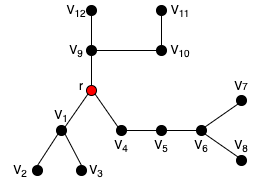
\includegraphics[width=0.5\textwidth]{12.png}
        \label{fig:figure-9}
    \end{figure}
    
    The leaves of the previous graph, with \(r\) as root, are \(\{v_{2},v_{3},v_{7},v_{8},v_{11},v_{12}\}\).
    
\end{document}
